\documentclass[12pt,a4paper]{scrartcl}
\usepackage[utf8]{inputenc}
\usepackage[ngerman]{babel}
\usepackage{amsmath}
\usepackage{amsfonts}
\usepackage{amssymb}
\usepackage{blindtext}
\usepackage{graphicx}
\usepackage{url}
\usepackage[style=alphabetic-verb,backend=bibtex]{biblatex}
\bibliography{bibliografie}
\usepackage{listings}
\usepackage[hidelinks]{hyperref}


\usepackage[left=2.5cm,right=1.5cm,top=3cm,bottom=2.8cm]{geometry}
\linespread{1.5}

\usepackage{fancyhdr}
\pagestyle{fancy}

\newcommand{\q}[1]{``#1''}

\begin{document}
\begin{titlepage}
\begin{center}

\vspace*{3cm}
\textbf{\huge{Projektarbeit}}\\
\vspace*{2cm}
\textbf{\large{Entwicklung eines 2D-Spiels mit SFML}}\\
\vspace*{5cm}
Gabriel Gavrilas, G3C\\
Jan Kunzmann, G3C\\
Patrick Eigensatz, G3C
\end{center}
\end{titlepage}


\clearpage
\newpage
\pagestyle{empty}
\mbox{ }
\clearpage

\setcounter{page}{1}
\section*{Vorwort}
Siehe auch in \cite{grundkurscpp}

\newpage

\tableofcontents

\newpage
\part{Dokumentation}
\section{Aufgabenstellung} 
Unsere Aufgabe ist eine Projektarbeit zu gestalten. Dazu hatten wir ein Semester Zeit. Man wählte ein Thema, dass einem intressiert. 
Zu dem eigen ausgewählten Thema muss man etwas erarbeiten. Den Lernfortschritt muss man in einem Lernprotokoll festhalten.
Dazu muss man eine Schriftlichearbeit abgeben und eine Präsentation machen. Diese Arbeit soll uns auf die Maturarbeit
vorbereiten.

\subsection{Motivation}
In unserer Generation verbringen viele Kinder, Jugendliche und Erwachsene
ihre Zeit mit dem Spielen von Computer- und Konsolenspielen.
Berühmte Vertreter sind Call of Duty, Grand Theft Auto und Minecraft.
Doch die meisten Nutzer dieser Programme haben nie die Prozesse hinter diesen verstanden.
Sei das wegen der bereits weit fortgeschrittenen Komplexität einiger Spiele
oder bei einfachen Spielen einfach die fehlende Motivation, sich damit zu befassen.\\
\\
Viele wollen nur wissen wie man ein Spiel spielt und nicht wie man es spielbar macht. Viele wissen nicht einmal wie schwer es ist schon ein
kleines Spiel zu machen.
Da wir selber auch zu dieser Generation gehören, 
machen wir alle immer wieder Erfahrungen mit den verschiedensten Games bzw. Spielen.
Doch wir wollten nicht blos Spiele spielen, 
sondern wir wollten selber ein Spiel entwickeln.
Dazu kam noch unsere Begeisterung für den Prozess des Programmierens.
Jeder von uns hatte bereits mehr oder weniger Erfahrungen auf diesem Gebiet gesammelt 
und wir waren und sind alle immer noch bereit mehr zu lernen.

\subsection{Persönliche Vorgaben}

Vor dem eigentlichen Projekt setzten wir uns selber einige Vorgaben.
\\
Uns war klar, dass ein Spiel auf dreidimensionaler Basis in der uns zu Verfügung stehenden Zeit nicht realisierbar war.
Dazu brachte die von uns gewählte Programmiersprache einige Hilfen mit sich, die wir bei der Entwicklung eines 2D-Spiels gut gebrauchen konnten.
\\
Um die Sache für uns attraktiv zu machen,
wählten wir bewusst eine Programmiersprache, die noch nicht
alle von uns beherrschten. Natürlich hätten wir genau so gut
SDL oder direkt das darunterliegende OpenGL verwenden können. OpenGL
schied aus, da der Aufwand bereits ein einfaches 2D-Spiel zu realisieren,
schlichtweg nicht möglich gewesen wäre. SDL war unser Favorit, bis wir
SFML entdeckten. Ganz im Gegensatz zu SDL schien SFML für C++ ausgerichtet
zu sein. So wurden Klassen anstatt Strukturen verwendet, was den (für den
Anfang komplizierten) Umgang mit Zeigern reduzierte. Ausserdem besitzen die
Klassen eigene Konstruktoren, bzw. Destruktoren, was das Initialisieren
oder das freigeben von Speicher überflüssig macht. Davon erhofften wir uns
weniger Speicherzugriffsfehler und ein schnelleres programmieren. SFML
überzeugte uns schlussendlich, als wir die in der offiziellen Dokumentation
gezeigten Beispielprogramme angeschaut haben. Zusätzlich wollten wir am Ende dieser Arbeit etwas in den Händen
haben.

\subsection{Ziele}
\begin{itemize}
\item 
Ziel unseres Projektes ist ein 2D-Einbrecherspiel zu entwickeln. Der Spieler soll eine Figur spielen, die in Häuser einbrechen muss und dort unentdeckt Gegenstände entwenden soll.
\item
Unser persönliches Ziel ist es, durch dieses Projekt, die Anwendung der Techniken der
Programmiersprache C++ zu lernen und zu vertiefen. Dies wollen wir durch
das Prinzip Learning-by-Doing erreichen. Jeder in der Gruppe soll am Ende
C++-Programme selber programmieren können.
\item
Wir setzen uns zum Ziel,
die Konzepte hinter Frameworks (namentlich SFML) zu verstehen und die
programmiertechnischen Abläufe hinter dem Spiel zu definieren und
umzusetzen.
\item
Wir wollen unser Spiel komplett im Team entwickeln und
mit dem Versionskontrollsystem git vertraut werden. Das alles soll uns später
für eigene Projekte und unsere Maturaarbeit helfen.
\item
Das Spiel muss/soll unter eine OpenSource Lizenz gestellt werden.
\end{itemize}


\newpage
\section{Begriffe}
\subparagraph{Game}
In dieser Dokumentation werden wir öfters auch den englischen und weit verbreitete Begriff \q{Game} an der Stelle von \q{Spiel} gebrauchen.

\subparagraph{Multimedia Framework:}
Eine Bibliothek mit Funktionen, die sich in C++-Programme einbinden lassen. Damit kann man verschiedene Aufgaben plattformübergreifend bewältigen und muss nicht alle Details selber programmieren.

\subparagraph{OpenSource Lizenz:}

Eine Lizenz, die das Einsehen, das Verändern und das Weiterverteilen des Quellcodes erlaubt.

\subparagraph{OpenSource-Software (OSS):}
Software, die unter einer OpenSource-Lizenz verfügbar ist.

\subparagraph{Versionskontrollsystem:}
Ein Programm, das Veränderungen an Dateien aufzeichnet und speichert, sodass mehrere Entwickler den Code gleichzeitig ohne Redundanz verändern können.

\subparagraph{GitHub:}
Für OSS-Entwickler von OpenSource kostenlose Plattform, um die über das Versionskontrollsystem git aufgezeichneten Veränderungen übersichtlich zugänglich zu machen.

\subparagraph{Travis CI:}
Für OSS-Entwickler kostenlose Plattform zur Qualitätssicherung: Kompiliert das Projekt automatisch nach jeder Änderungen und führt Tests durch, um zu sicherzustellen, dass das Programm einwandfrei funktioniert.

\subparagraph{Coverity:}
Für OSS-Entwickler kostenlose Plattform: Führt eine tiefgreifende statische Quellcodeanalyse durch, und hilft so Programmierfehler zu vermeiden und zu finden.

\section{Entwicklungswerkzeuge}
\subsection{Simple and Fast Multimedia Library}
\textbf{SFML}, kurz für \q{Simple and Fast Multimedia Library}, ist ein Multimediaframework, das wir hier quasi als
\q{Entwicklungswerkzeug} definieren, obwohl es eben ein Framework ist, das wir in unserem Programm verwendeten. SFML
liefert viele Klassen, die in verschiedenen Modulen (\textit{Sound}, \textit{Graphics}, \textit{Network}, ...) inkludiert
und ins Programm gelinkt werden können. Diese Module sind bewusst plattformübergreifend entwickelt worden, so dass wir uns
nicht um eine Portierung des Spiels kümmern mussten.
\\
\\
SFML war quasi die Schnittstelle zwischen unserem Modell des Spiels im Arbeitsspeichers, und dem Benutzer des Spiels. Ein Beispiel:
Wir wussten, wo sich der Spieler auf der Ebene befindet, und wir konnten mit SFML eine Bilddatei als Textur laden, und diese
an der Position des Spielers aufzeichnen lassen. Über SFML konnten wir auch die Tastatur einlesen sowie Musik abspielen.

\subsection{Code::Blocks}
Code::Blocks ist eine frei verfügbare Entwicklungsumgebung (IDE\footnote{Integrated Development Environment}) die Programmierung in C/C++ und D.
Neben der Syntaxhervorhebung und der intelligente Autovervollständigung bietet Code::Blocks bequeme Einstellungen um SFML-Projekte auf allen Plattformen
einfach zu kompilieren. Code::Blocks setzt dabei auf eine Art \textbf{make}, wie es schon aus Unixzeiten bekannt ist. Kompiliert wird nur das, was sich
seit dem letzten Durchgang geändert hat. Code::Blocks nutzt \textbf{g++}, den GNU C++ Compiler, um die einzelnen Dateien in Objektcode umzuwandeln und diesen
anschliessen in eine ausführbare Datei zu linken.

\subsection{git und GitHub}
\textbf{git} ist eine sogenannte verteilte Versionskontrolle (DVCS\footnote{Distributed Version Control System}). Ein solches Werkzeug übernimmt
den Entwicklern einige Arbeit, wenn es darum geht, parallel an Software zu schreiben. Zudem zeichnet es alle Änderungen am Code auf und man kann diese
einsehen, um zum Beispiel Fehler zu finden, sie erst seit kurzem vorhanden sind, oder gewisse Änderungen rückgängig zu machen, ohne dass man
manuell die Dateien zerpflücken muss. git überzeugte uns durch seine Einfachheit, seine Effizienz und seine Möglichkeiten. git erwies sich
als enorme Hilfe, sei es um Fehler zu finden oder einfach zum Programmieren.
\\
\\
\textbf{GitHub} ist ein
Onlineportal, das das Hosting von Projekten, die mit git verwaltet werden, kostenlos übernimmt. Das Projekt erhält eine eigene Übersichtsseite,
die ebenfalls zur Entwicklung genutzt werden kann, und auf der Interessierte den Code und die Änderungen einsehen können. Wir haben GitHub nicht nur
als Hoster genutzt, sondern ebenfalls, um unsere Termine und Fristen mit dem Projektkalender festzulegen.
\begin{figure}
\centering
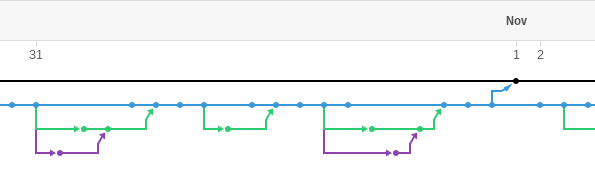
\includegraphics[scale=1]{img/branches.png}
\caption{Verschiedene Entwicklungszweige zur parallelen Entwicklung auf GitHub}
\label{fig:branches}
\end{figure}


\subsection{Coverity Scan}
\textbf{Coverity Scan} ist der Name eines Produktes der gleichnamigen amerikanischen Firma. 2006 erhielt diese Firma vom US-Verteidigungsministerium
einen finanziellen Zuschuss, um es für OpenSource-Projekte kostenlos möglich zu machen, ihren Code auf Sicherheitslücken und Programmierfehler untersuchen
zu lassen. Dabei funktioniert Coverity keines Wegs wie ein normaler Compiler (erkennt also keine syntaktischen Fehler wie das Fehlen eines Semikolons),
sondern es versucht den Code zu verstehen und mögliche semantische Fehler zu finden. So werden Entwickler hingewiesen, dass zum Beispiel eine Funktion
unter gewissen Bedingungen nie terminiert und so das Programm blockiert. Auch findet Coverity schnell Speicherlecks und Speicherzugriffsfehler.
Während der Entwicklung haben wir unser Projekt regelmässig von Coverity überprüfen lassen.
\begin{figure}
\centering
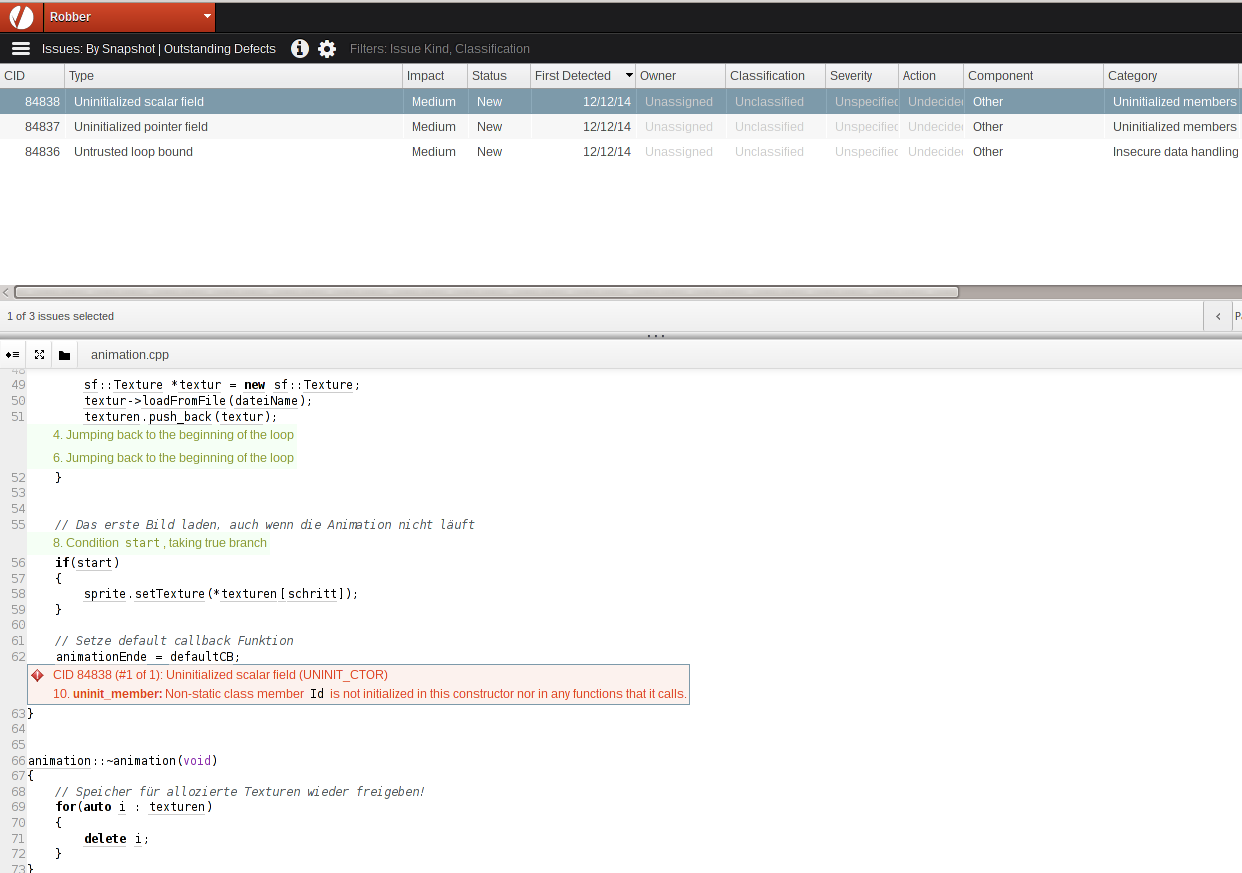
\includegraphics[scale=0.4]{img/coverity.png}
\caption{Coverity hat 3 Fehler gefunden und markiert die fehlerhafte Stelle im Code}
\end{figure}

\subsection{Valgrind}
\textbf{Valgrind} ist ein freies Programm zur dynamischen Fehleranalyse in Programmen. Besonders nutzten wir die Fähigkeit,
unser Spiel innerhalb des Memcheck-Moduls laufen zu lassen, um ein Feedback über den Speicherverbrauch zu erhalten. So entdeckten
wir, dass viele Klassen, die schnell erstellt wurden, zwar Speicher anfordern, diesen aber nie mehr freigeben. Das führte schlussendlich
zu einem Speicherleck von knapp 20MB,
 das schliesslich behoben werden konnte.

\begin{figure}
\centering
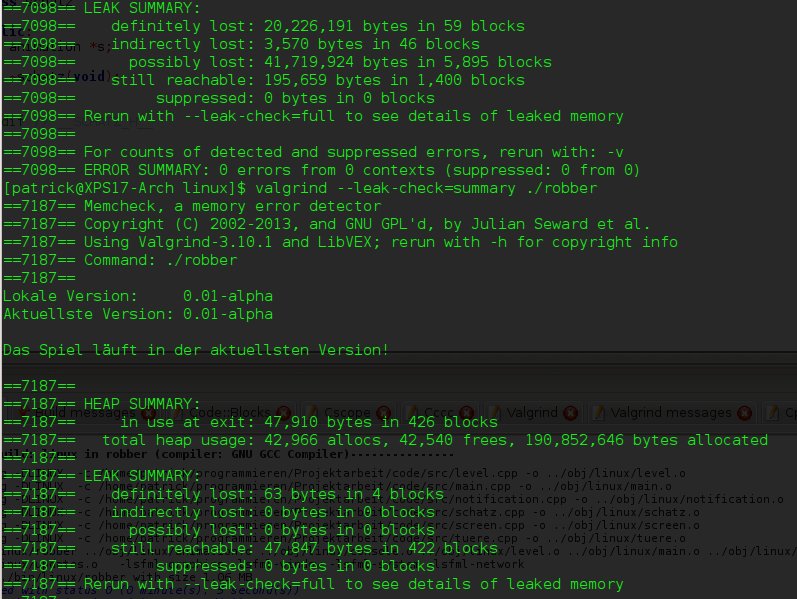
\includegraphics[scale=0.8]{img/valgrind2.png}
\caption{Valgrinds Memcheck}
\end{figure}


\subsection{GIMP}
Ein Programm um Bilder zu bearbeiten oder auch selber Bilder zu erstellen. 
\subsection{GDB - Der GNU Debugger}

\newpage
\section{Vorgehen}
\subsection{Vorbereitung}
\subsubsection{Spielidee}
Am Anfang stand ganz klar die Ideenfindung auf dem Programm. Es war uns wichtig,
eine Spielidee zu finden, an der ein Spieler später auch Spass haben würde,
und wir das Spiel je nach zeitlichen Kapazitäten auch etwas erweitern könnten.
Diese drei Fragen halfen uns:
\begin{itemize}
\item Würdest du das Spiel spielen?
\item Ist das Spiel technisch überhaupt realisierbar?
\item Ist das Spiel erweiterbar?
\end{itemize}
Der Ideenfindungsprozess dauerte mehrere Wochen, es war nicht einfach, eine Idee
zu finden, die uns alle begeistern würde. 
Als wir genug Ideen hatten, fertigten wir eine Liste an. 
Wir setzten uns ein Zeitlimit von einer Woche, um zu jeder Idee jeweils einen Umsetzungsvorschlag zu erstellen. 
Dadurch hatten wir zu jeder Idee 3 verschiedene Vorschläge.
Dadurch und durch weitere Diskussion kamen wir auf die Idee eines Eibrecherspiels.
Dieses erfüllte alle Vorgaben:
Die Idee fanden wir alle interessant, es war mit unseren Mitteln und unserem Wissen realisierbar und man kann es gut erweitern.

\subsubsection{Vorbereitung und Planung}
Parallel zur Ideenfindung haben wir uns - wie in der
Disposition vermerkt - intensiv mit der Programmiersprache C++ beschäftigt. Das Einarbeiten
in die Sprache war sehr zentral für das spätere Verständnis der SFML-Bibliothek, die uns
unter Anderem das Anzeigen von Grafiken ermöglichte.
\\
Bevor wir nun jedoch mit dem Programmieren anfangen konnten, mussten wir die Idee ausarbeiten.
Sicher war zuerst nur, dass es ein zweidimensionales Spiel sein wird und das Thema Einbrechen werden soll.
Darum begannen wir das Spiel zu porträtieren. 
Das leeren eines Hauses sollte das Ziel sein, wobei wir damals noch 3 verschiedene Spielmodi geplant hatten:
\begin{itemize}
\item Einen bestimmten Gegenstand klauen
\item In einer bestimmten Zeit, so viel wie möglich stehlen
\item Einen möglichst hohen Wert der gestohlenen Waren erreichen
\end{itemize}
Bei den Grafiken einigten wir uns auf Einfachheit, denn es ist kein zentraler Punkt unseres Spieles.
Bereits in diesem Stadium besprachen wir auch mögliche Probleme beim Programmieren und dem Aufbau des Programms.
Dabei wurden die Grundsteine für wichtige Elemente unseres Programms gelegt: Kollisionsdetektion, Teleportieren, Schätze oder auch die Loops, auf denen unser Spiel basiert. 
Durch diese vorhergehende Fehlersuche hatten wir bereits Lösungen zu einigen Problemen, auf die wir treffen würden. Diese konnten wir dann bequem umgehen oder mussten feststellen, dass einige Problem komplexer sind als wir damals noch dachten.
Der nächste Punkt war das Umsetzen unseres gesammelten Wissens und damit das Erstellen des Programms.

\subsubsection{Umsetzung}
Wir haben uns immer wieder Stichtage festgelegt, so dass wir immer gewisse Ziele erreichen mussten. So konnten wir unsere Planung grob einhalten. Jeder hat immer wieder gewusst was man als nächstes machen muss. Falls jemand mal ein Problem hatte. Hat es eine kleine Problemlösungsrunde gegeben, bei der jeder versucht hat nur das Problem zu lösen und so konnte speditiv weiter gearbeitet werden. So sind wir Schritt für Schritt vorwärts gekommen. Es hat auch immer wieder Verbesserungen oder Abänderungen gegeben am alten Code. So dass der Code jetzt möglichst einfach und optimal ist. 

\newpage
\subsection{Das Programmieren}
\subsubsection{Das Laden erster Grafiken}
Unsere erste Version des Spieles war bloss ein Fenster mit der Hintergrundgrafik.
Zu allen Dingen haben wir zuerst Demografiken gebraucht.
Obwohl dieser Schritt einfach erscheint kam dabei eines unserer grössten Probleme in der Entwicklung des Spieles zum Vorschein.
Die Schwierigkeit war es, dass diese erste Version bei allen gleich aussieht, unabhängig von Auflösung, Marke oder Betriebssystem.
Weiteres zu diesem Problem gibt es im Kapitel \ref{aufloesungsprobleme} auf Seite \pageref{aufloesungsprobleme}.


\begin{figure}[h]
\centering
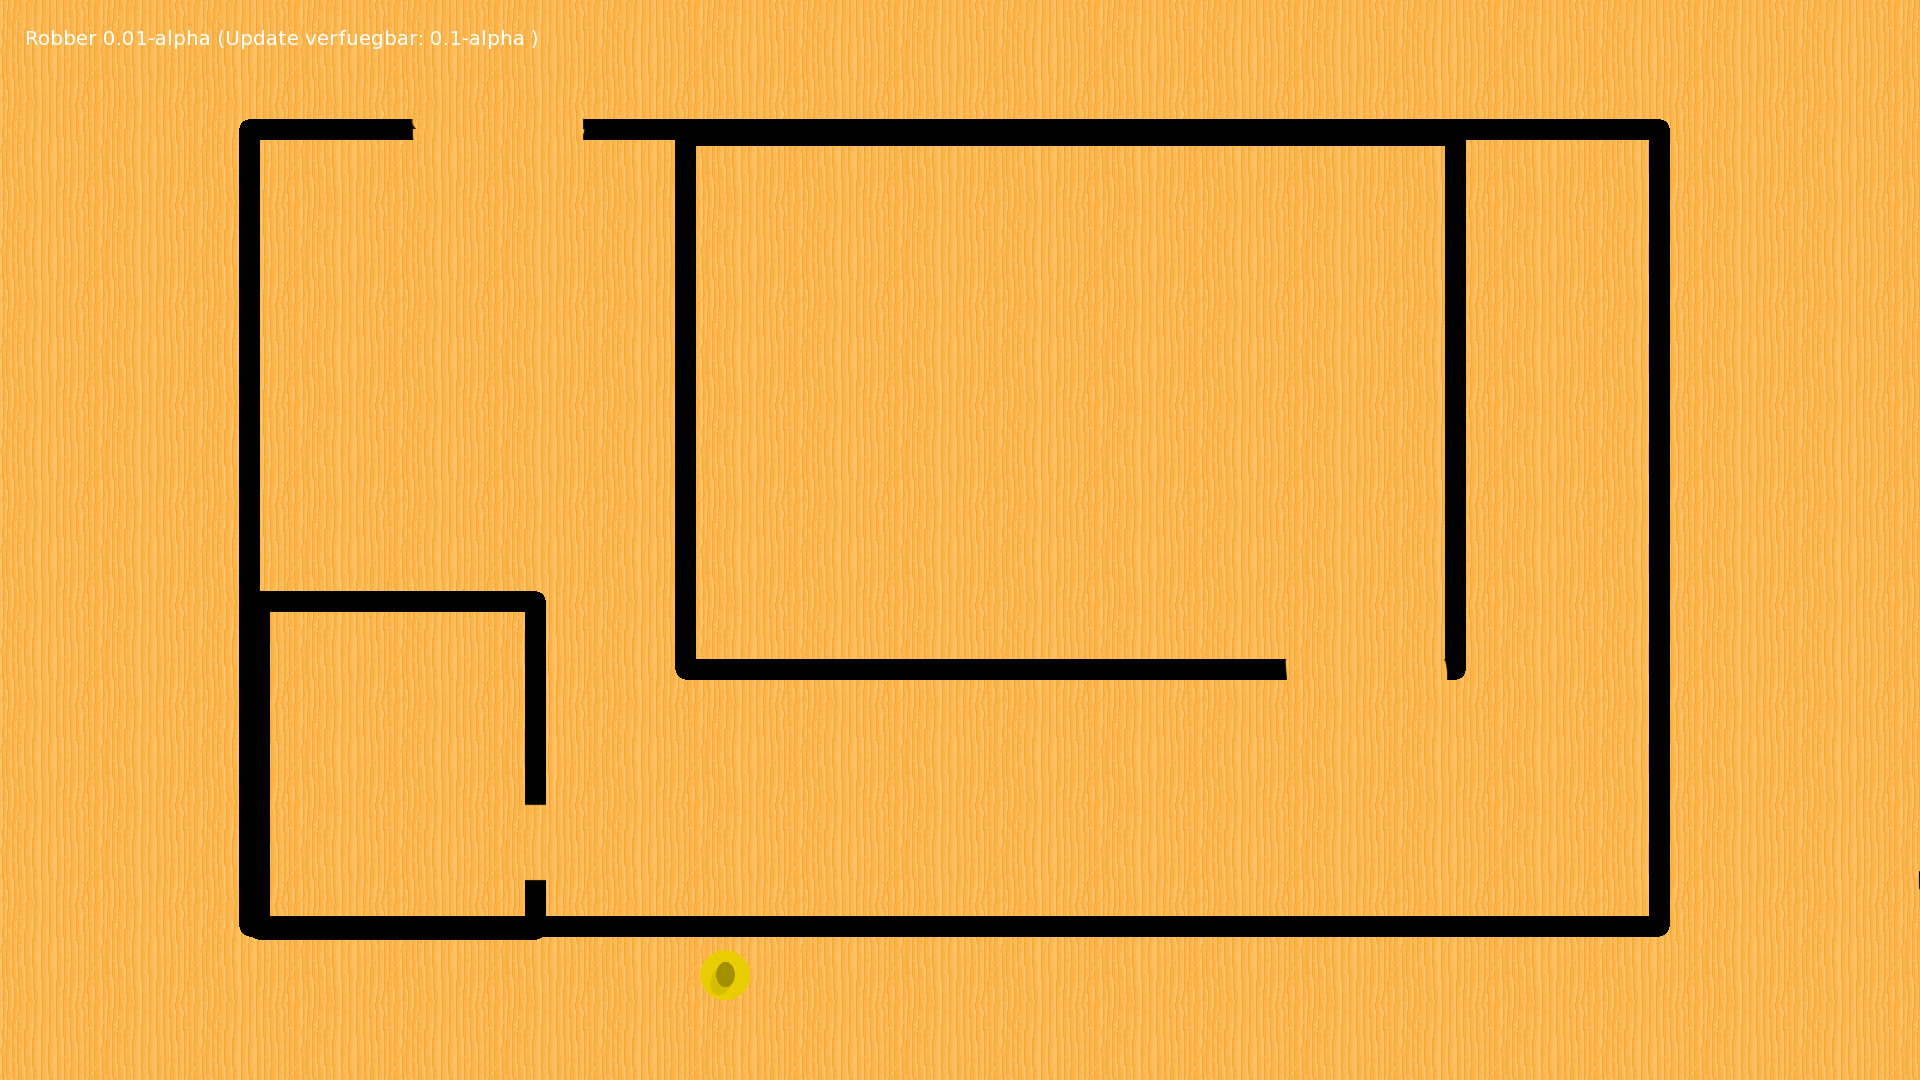
\includegraphics[scale=0.25]{img/grafiken.png}
\caption{Ein Beispiellevel mit der Spielfigur}
\end{figure}


\subsubsection{Überprüfung auf Updates}
Versionsdatei von GitHub geladen, wenige Bytes, überprüfen und entsprechende Meldung im Spiel.
Wird noch ausgedeutscht.

\subsubsection{Kollisionsdetektion}
Wir haben uns entschieden die Mauern von Anfang an auf den Hintergrund zu zeichnen. Dann machen wir ein FloatRect, ein Quadrat,
über jede gezeichnete Mauer. Die Kollisionsdetektion ist da um zu erkennen ob der Spieler in eine Mauer läuft.
Diese war zu Beginn der Entwicklungen etwas fehleranfällig. So gab es vereinzelt
Schlupflöcher ganz geringer Breite, sodass man durch die Mauer wandern konnte. Neben der Mauer hingegen,
versteckte sich eine unsichtbare Mauer, das heisst, es wurde eine Kollision gemeldet, obwohl an der
Spielerposition gar keine Mauer lag. Um das Problem zu Erforschen und schliesslich zu beheben, haben
wir die Mauerabschnitte einzeln geladen und ein grünes Rechteck darübergezeichnet. So fiel uns auf, dass
die Koordinaten der Mauer zwar richtig gelesen, aber falsch verarbeitet wurden. Die Koordinaten mussten
von absoluten Bildschirmkoordinaten in Fenster/Spielkoordinaten umgerechnet werden. Das konnte wir nach einigem ausprobieren beheben.

\begin{figure}[h]
\centering
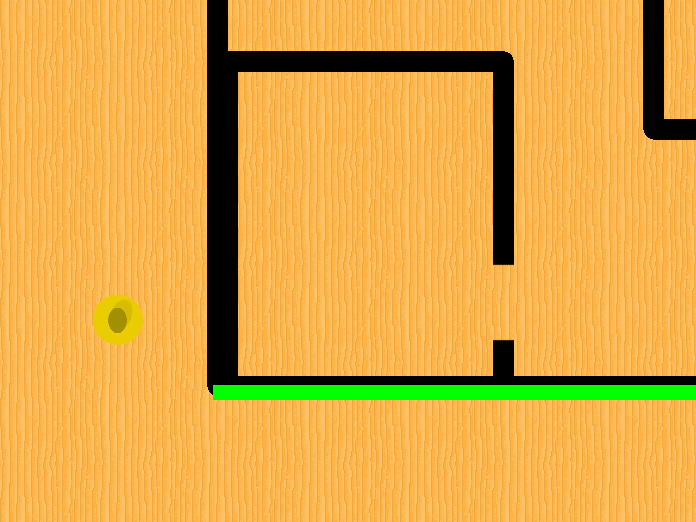
\includegraphics[scale=0.3]{img/kollisionsdetektion.png}
\caption{Debugging der Kollisionsdetektion}
\end{figure}

\subsubsection{Levelclass und Leveldatei}
Unser Ziel war zuerst ein Probe Level zu haben, es dann aber einfach zu haben ein richtiges Level zu erstellen. Deshalb haben wir uns entschieden, dass wir zu jedem Level eine Leveldatei machen, in der alle variablen informationen 
enthalten sein müssen. So steht dort immer zuerst wie viele, dass es von diesem Obejekt hat und dann oft noch die genaue 
Position. SO stehen die Mauer oder auch die Pfeile dort vermerkt. Es steht auch zu welchem Level gejumpt werden soll wenn 
man auf einen Pfeil kommt.
Dies wird in der Leveclass alles genau heraus gelesen. Das wichtige dabei ist, dass die Reihenfolge genau stimmt sonst gerät 
das ganze in ein irres Durcheinenader. Wir brauchen die Anzahl Elemente die es hat zuerst, um zu erkennen welche Information 
zu welchem Objekt gehört. Denn das Programm liesst dort nur Zahlen heraus. Und mit Wörtern können wir ihm das nicht erklären, 
da er diese ja nicht verstehen kann.

\begin{figure}[h]
\centering
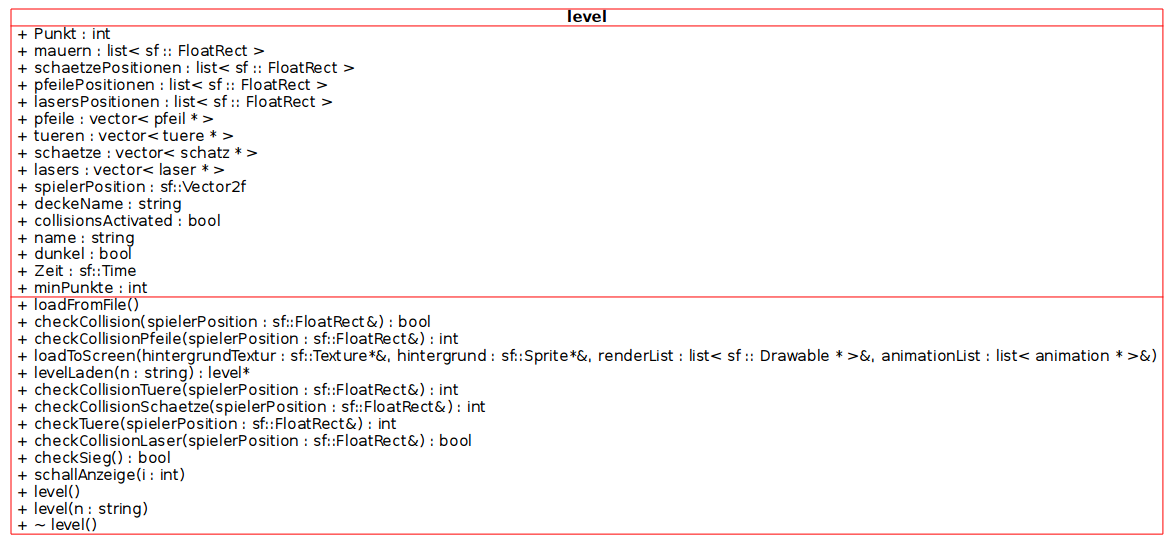
\includegraphics[scale=0.45]{img/level_uml.png}
\caption{UML der Levelklasse}
\end{figure}


\subsubsection{Animationen}
Von Anfang an waren auch Animationen in unserem Spiel eingeplant. So sollen zum Beispiel ausserhalb eines Hauses
Türen durch grün blinkende/aufleuchtende Pfeile markiert werden. Für solche Animationen wurde eigens eine Klasse
implementiert.
\begin{figure}[h]
	\centering
	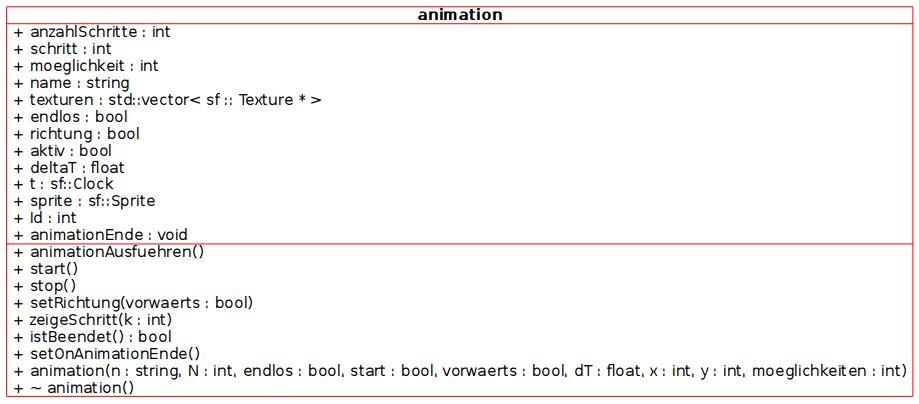
\includegraphics[scale=0.6]{img/animation_uml.png}
	\caption{UML der Animationsklasse}
\end{figure}
Um Animationen später oft und möglichst einfach verwenden zu können, besitzt die Klasse einen einfachen Konstruktor,
der die Bilder bereits lädt, die Position und die Zeitspanne $\Delta t$ zwischen den einzelnen Bildern festlegt.
\begin{figure}[h]
	\centering
	
\includegraphics[scale=0.3]{img/animation_pfeil.png}
	\caption{Die erste Animation im Spiel: Ein blinkender Einstiegspfeil}
\end{figure}
Innerhalb unserer $main()$-Funktion nützten wir eine $std::list<animation *>$ Liste aus der STL\footnote{Standard Template Library}.
Bevor die Sprites in das Fenster gezeichnet werden, werden die Texturen der Sprites dem Animationszeitpunkt entsprechend
neu geladen. So entsteht das Gefühl einer Bewegung, bzw. hier Anpassung der Farbe. Entscheidend ist dabei die Methode
$animationAusfuehren()$, die überprüft, ob bereits genug Zeit vergangen ist, das neue Bild anzuzeigen und dies gegebenenfalls
übernimmt.


\subsubsection{Pfeile}
Zuerst haben wir geplant die Pfeile nur als Anzeiger zu nutzen, wo dass Eingänge sind. Doch dann hatten wir die Idee, dass man sie auch gleich als Teleporter benutzen könnte. SO standen wir vor einem viel schwereren Herausforderung. Wir haben dies dann so gelöst, dass wenn man auf den Pfeil kommt wir aus der Lveldatei gelesen, welches Level geladen wrden soll. Bei der Anzahl Pfeile steht dann wie viele Pfeile es hat. Zuerst wo sie sind und mit welcher Rotation. Dann hat es noch 2 Zahlen, diese geben die neue Starposition der Figur im neuen Level an. Dies könnte man dann auch benutzen und ausbauen, so dass wir Häuser mit mehreren Etagen bilden könnten. WIr haben noch Rote Pfeile gezeichnet um Ausgänge aus dem Haus zu kenzeichnen. Durch eine weitere Zahl in der Leveldatei werden entweder die roten oder die gelben Pfeile geladen.

\subsubsection{Console}
Wir haben eine Console eingebaut, die sich mit der rechten Shift-Taste öffnen lässt. In dieser kann man verschiedene kleine Hilfen aktivieren. Wie zum Beispiel, dass man durch Mauern und Türen gehen kann. Man kann aber auch das Level direkt wechseln.

\subsubsection{Tastatur}
Man kann die Figur mit den Tasten W, A, S und D bewegen. Mit der Taste W geht die Figur nach oben, mit A nach links, mit S nach unten, mit D nach rechts. Hier können wir im SFMl auf eine einfache Form zurückgreifen. Diese erkennt, ob und welche Taste gedrückt wird. So konnten wir jeder Taste einen gewissen Befehl zuordenen und genau sagen was getan werden soll. Zum Beispiel bei der Taste W steht, dass sich die Figur um -5 bewegen soll. Dies bewirkt eine Bewegung nach oben. Da das Koordinatensystem bei jedem Laptop oben links mit 0/0 beginnt und dann nach unten negativ wird. Bei den anderen Tasten gibt es nur einen leicht anderen Befehl aus der SFML Klasse. 	+ Man kann die Figur mit... to be continued
Bei diesen Tastenabfragen wird auch gleich überprüft, ob an in eine Mauer läuft, sollte dies nähmlich der fall sein darf sich die Figur ja nicht bewegen. Deshalb machen wir in diesem Fall das ganze wieder rückwärts. Wir haben auch einen Sprint eingebaut. Dazu muss man dir linke Shift Taste drücken und sich bewegen. Dann bewegt sich die Figur doppelt so schnell. Jedoch wird der Schalpegel erhöt (Verweis). Dies haben wir mit einer Variabel gemacht, so ändert sich die Variable je nach dem ob die Taste gedrückt wird oder nicht. 	
Mit den Zahlentasten 9 und 0 kann herein und heraus zoomen. Da haben wir aber noert werden kann. Wir haben einen mindest Zeitabstand eingebaut, so dass sich die Tür erst wieder nach einer gewissen Zeit schliessen lässt. Sonst hätte man die Türe schneller öffnen und schliessen können als das Spiel mithalten könnte und würde die Tür noch oft öffnen und schliessen.Wir haben die Türen noch etwas grösser gemacht bei der Collisions-Abfrage, so dass man die Türen schlussendlich immer von beiden Seiten öffnen und schliessen kann. 	
 	
 	
\subsubsection{Das Hauptmenü} 	
Das Hauptmenü wurde bewusst relativ simpel gehalten und konnte dadurch sehr schnell erstellt werden. Mit GIMP wurden 	
einige mehr oder weniger gut aussehende Grafiken erzeugt, die als Buttons verwendet werden konnten. Doch da wir hier wieder auf ein Problem mit den Koordinaten stiessen entschieden wir uns unser Game nicht, wie viele andere aufzubauen. Nun ist man bereits im Hauptmenu die Spielfigur und da hatten wir es leicht. Wir haben einfach das Spielstarten Bild als neuen Pfeil definiert falls eine 2 in der Leveldatei steht. So ist es, sobald man auf das Spielstarten fährt einn Teleporter zum ersten Level. Bei der Spielbeenden haben wir ein FloatRect erstellt und eine checkCollison gemacht und falls der Spieler nun auf Spielbeenden fährt beendet das Spiel. 	
 	
 	
\subsubsection{Dunkle Level} 	
Mit einem halbtransparenten Overlay können wir das Level, bzw. das Haus abdunkeln, und nur in einem Bereich um uns 	
sichtbar machen. In der Leveldatei wird eingetragen, ob ein Level dunkel, oder hell ist. Dementsprechend wird dann das 	
Overlay geladen oder nicht. Das führt zu spannenderen Spielen, weil man Gefahren und die Schätze relativ spät sehen kann. 	
Besonders beim Spiel auf Zeit entsteht so quasi ein zusätzlicher Druck. 	
 	
\subsubsection{Musik} 	
Wir haben einen Kolleg angefragt, ob es ihm etwas ausmachen würde, Musik für uner Game zu machen. Er war damit einverstanden und hat uns Musik komponiert. So dass unser Game jetzt auch Hintergrundmusik laden kann. Er hat 3 verschiedene Stücke komponiert. Eines für das Hauptmenü, eines für die Leveln und das Letzte für das Game Over. Nun wir haben das so gelöst, dass wir den Namen der Leveldatei überprüfen und dass es dann je nach Name eine andere Musik lädt und abspielt. Dies hat praktisch auf anhieb funktioniert. 	
	
\subsubsection{Schallpegel} 	
Wir haben auch einen Schallpegel eingeführt. So kann man nicht nur von den Lasern geschnappt werden. Sondern man kann auch zu viel Lärm machen und so geschnappt werden. Damit man sieht wie knapp es ist, hat es eine Anzeige links, bei der der Schallpegel steigt und sinkt. Wenn man im roten bereich angekommen ist, wird eine zufällige Zahlgewählt, bei der man zu laut ist. Diese Zahl liegt zwischen 1 und 200. So wollen wir dem ganzen ein bisschen mehr Spannnung verleihen. Man macht mehr lärm, wenn man rennt oder eine Tür öffnet. Nach gewisser Zeit senkt sich der Pegel jedoch wieder. Die Grafik haben wir mit einer Animation eingeführt. Sie wird nur bei den Dunkelleveln angezeigt, da man nur bei diesen leise sein muss.
 	
\begin{figure}[h] 	
\centering 	
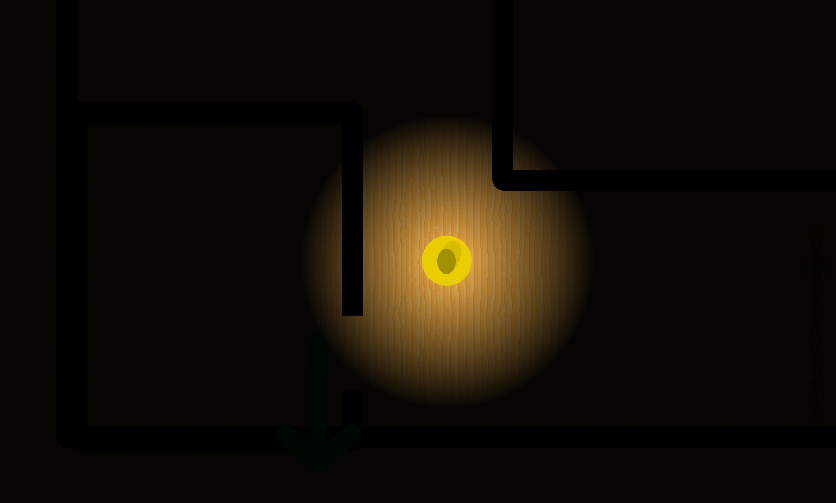
\includegraphics[scale=0.5]{img/dunkel.png} 	
\caption{Ein dunkles Level} 	
\end{figure} 	
 	
\subsubsection{Punkte} 	
Wir haben ein Punktesystem eingeführt. Jeder Schatz gibt einem 10 Punkte. In der Leveldatei wird angegeben, was die Punktzahl ist, die man erreichen muss. Sobald man diese Punktazhl durch sammeln der Schätze hat, gerät man automatisch ins Hauptmenu. Später wäre der Sinn, dass man dann ins nächste Level kommt. Die Punkte werden oben links auf dem Bildschirm dargestellt. 	
 	
\subsubsection{Zeit} 	
Wir haben auch eine Zeit eingebaut. So läuft die Zeit Obenlinks langsam herunter und falls man nicht durch das Level gekommen ist, Fällt man aus dem Spiel ins Gameover. Die zur verfügung stehenden Zeit wird in der Leveldatei geschrieben.	
 	

\subsection{Wahl der Spielarchitektur}
Als wir die Grundlagen von C++ zusammen erarbeitet hatten, mussten wir natürlich vorausplanen, wie wir das Spiel programmieren würden.
Wir kannten zwar Verzweigungen, Schleifen und Funktionen, aber wie können wir damit ein Spiel entwickeln? Auf Seite 106 in \cite{sfml_gamedev} 
wird eine parallele Spielarchitektur erwähnt. Wir fanden die dort beschriebene Spielarchitektur aber unnötig komplizierter und erarbeiteten uns
dann eine andere Struktur. Daraus resultierte die Struktur in Abbildung \ref{fig:seriell}.
die wir mit der Zeit auch implementiert hatten.\\
\begin{figure}[h]
\centering
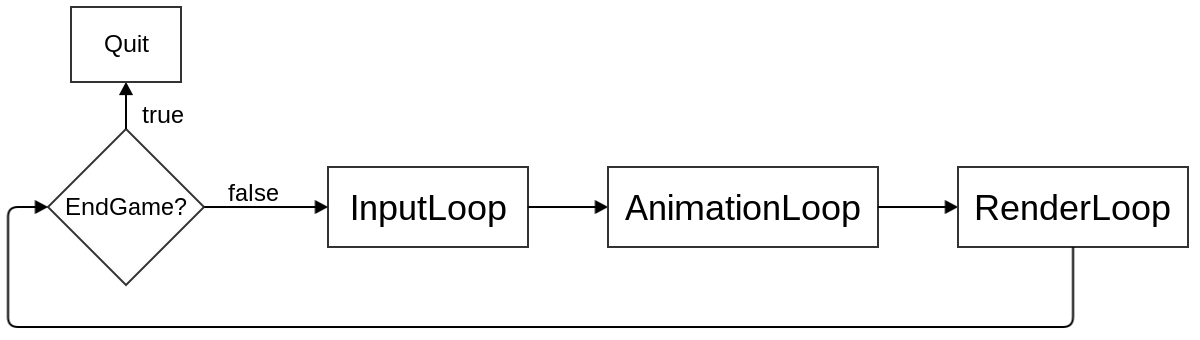
\includegraphics[scale=0.3]{img/gameloops.png}
\caption{Unsere serielle Spielarchitektur}
\label{fig:seriell}
\end{figure}

\subsubsection{Serielle Architektur}
Die serielle Architektur unterteilt sich in vier Teile, die immer vollständig und immer hintereinander ablaufen. Die Funktionsweise
und die Aufgaben der Teile werden hier kurz erläutert:\\
\\
\textbf{EndGame?}
Diese Abfrage überprüfte nur, ob das Spiel beendet werden muss, sei es aufgrund eines Fehlers im Spiel
oder weil der Benutzer das Fenster schliessen wollte.\\
\\
\textbf{InputLoop}
Dieser Teil ist dafür zuständig, die Eingaben des Spielers zu einzulesen, und aufgrund von den Eingaben Aktionen auszulösen. Wenn zum Beispiel
der Spieler bei einem Schatz in der Nähe steht, und die Taste $[E]$ drückt, werden dem Spieler 10 Punkte gutgeschrieben und der Schatz muss beim
RenderLoop entfernt werden, damit er beim nächsten Durchgang verschwindet. Steht der Spieler bei einer Türe und drückt $[E]$, dann wird die Animation
der Türe gestartet und die Mauer der Türe muss umplatziert werden. Wenn sich der Spieler in den Strahl einer Lichtschranke bewegt, wird das Level
\q{Game Over} geladen.\\
\\
\textbf{AnimationLoop}
Hier wird für jede Animation überprüft, ob sie überhaupt aktiv ist, und wenn ja, ob seit dem letzten Durchgang bereits die für jede Animation
eigene Zeit $\Delta t$ verstrichen ist, damit dem Sprite die nächste Textur zugeordnet werden kann.\\
\\
\textbf{RenderLoop}
Die einzelnen Sprites werden in das SFML Fenster gezeichnet, und SFML wird angewiesen das Fenster neu auf den Bildschirm zu \q{zeichnen}.

\subsubsection{Parallele Architektur}
SFML unterstüzt mit der \textit{Thread}-Klasse eine plattformübergreifende Implementierung
von Systemthreads. Wenn ein Thread erstellt wird, springt das Programm an diesem Punkt
in eine Funktion und führt diese parallel zum Rest des Programmes aus. Der grosse Vorteil,
der sich dadurch ergibt, ist sicher die Performance, also die Ausführgeschwindigkeit. Die
parallele Architektur würde sich demnach in drei bis vier Teile aufgabeln, je nachdem, ob man die AnimationLoop
und die RenderLoop in jeweils einzelne Threads nimmt oder nicht. Da wir
nicht wussten, dass SFML so effizient arbeiten würde, und unser Spiel auch ohne parallelen Code
ohne Ruckler spielbar wäre, hatten wir unsere Spielarchitektur ursprünglich so geplant:
\\
\begin{figure}[h]
\centering
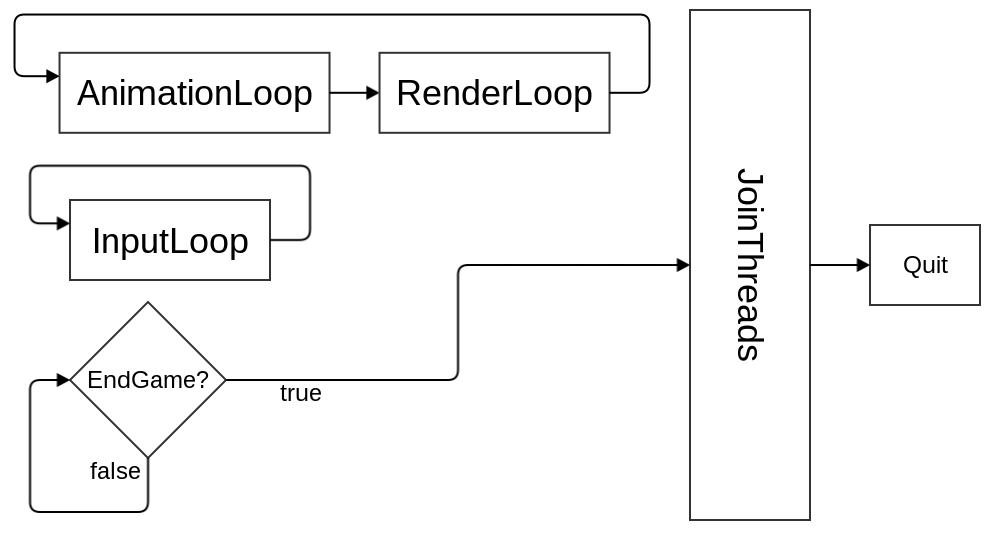
\includegraphics[scale=0.3]{img/threads.png}
\caption{Die parallele Spielarchitektur}
\end{figure}


\section{Probleme und Lösungen} 	
\subsection{Auflösungsproblem XY} 	
\label{aufloesungsprobleme} 	
Beim Auflösungsproblem handelt es sich um ein Problem mit dem Umgang mit SFML. 	
Das Problem besteht darin, dass jede Ansicht bei jeder Auflösung, jeder Gerätemarke und bei beiden Betriebssystemen gleich aussehen ch gewisse Probleme (verweis) 	
Die Taste E ist die Taste für alles was man bewegen kann. So wird dort überprüft, ob es eine Tür hat und falls ja, dann öffnet oder schliesset es diese. Dazu muss es aber auch die erstelten Mauern aus der RenderList löschen und eine neue Mauer hinein geben. und weil es so viele möglichkeiten gibt die Tür zu öffnen muss es jede abrufen könnnen, was einen erheblichen rechenaufwand dargestellt hat. Aber man kann mit E auch den Schatz aufnehmen.
\label{aufloesungsprobleme}
Beim Auflösungsproblem handelt es sich um ein Problem mit dem Umgang mit SFML.
Das Problem besteht darin, dass jede Ansicht bei jeder Auflösung, jeder Gerätemarke und bei beiden Betriebssystemen gleich aussehen soll.
Wir hofften, dass SFML diese Arbeit übernehmen würde, doch bereits bei den ersten Grafiken mussten wir einsehen, dass wir alles selber regeln müssen.
Um das Problem zu lokalisieren benutzten wir die $zoom()$-funktion, mit der man die ganze Ansicht über einen Wert anpassen kann.
Diesen Wert nannten wir factor.
Diesen factor bestimmten wir durch den Quotienten aus Auflösung und Ansichtsgrösse.
\begin{quote}
Eine View ist eine Klasse der SFML Bibliothek.
Man kann es sich als eine 2D-Kamera vorstellen, die definiert, welche Region des Bildes angezeigt wird.
Wir haben die View für unser Spiel Ansicht genannt.
\end{quote}
Wir erhofften uns ,durch annähern der richtigen Grösse des factors, eine Gesätzmässigkeit zu finden.
Schnell wurde uns jedoch bewusst, dass diese Lösung längerfristig nicht haltbar war,
denn dies führte auch dazu, dass zum Beispiel die Mauern umgerechnet werden mussten.
Nicht nur war der Aufwand zu gross, sondern brachte es auch weitere Probleme mit sich.
Beim Einführen der Mauern waren sie nicht, wie zuvor beim Hintergrundbild, 
bei allen gleich, sondern an unterschiedlichen Orten.
Durch weitere Tests konnten wir den factor so verändern, dass auch dies nicht mehr vorkam.
Doch weitere Versuche zeigten, dass die Mauern im allgemeinen nicht richtig verrechnet wurden.
Schlussendlich mussten wir feststellen, dass das Problem so nicht zu lösen war.
\\
Das Problem war die Handhabung von drei verschiedenen Koordinatensystemen.
SFML regelt seine Grafiken mit zwei Koordinatensystemen.
Das erste hatte das Zentrum im linken oberen Ecken des Bildschirms und gibt jedem Pixel des Bildschirms eine Koordinate. 
Die Ansicht ist an dieses System gebunden.
Das zweite System hat seinen Zentrum im virtuellen oberen Ecken der Grafiken. 
Von dort werden die Positionen der Grafiken innerhalb des Fensters bestimmt. 
Dieses System ist frei von der Ansicht, diese kann sich frei über dieses System bewegen.
Über vordefinierte Funktionen der SFML Bibliothek konnten wir diese ineinander umrechnen.
Wir selber haben durch den factor ein eigenes, neues System erstellt.
Viel Zeit ging verloren, beim verstehen der Zusammenhänge dieser Systeme, vor allem unseres Eigenen.
\\
Durch das verankern der Ansicht auf den Spieler, konnten wir die Arbeit mit dem factor umgehen und ihn wieder herausstreichen.
Diese Variante gefiel uns auch besser, denn wir gingen nie von immer gleich grossen Levels aus, was beim factor ein grosses Problem gewesen wäre.
\\
Wie bereits erwähnt regelt SFML das Anzeigen mit zwei Koordinatensystemen.
Dies ist die einzige Fehlerquelle die noch besteht.
Hier gibt es einen Fehler einerseits bei der Bestimmung der Auflösung des Bildschirms und andererseits in der Umsetzung im Spiel.
Dadurch kam und kommt es auf wenigen Bildschirmen mit hoher Auflösung zu Anzeigefehler.
Dafür haben wir auf die zoom()-Funktion zurückgegriffen, doch dieses mal ist der Wert während dem Spiel manipulierbar und hat eine Beschränkung.
Wir können Fehler bei dieser Funktion nicht ausschliessen, doch haben wir uns entschlossen diese nicht mehr zu verändern.

\subsection{Compilerprobleme}
Nicht nur wir machten Fehler bei der Entwicklung, und die Fehler von anderen sind erfahrungsgemäss schwerer aufzuspüren.
Einem eher speziellen Problem begegneten wir, als wir den Pfad für ein Animationsbild erstellen wollten.
Die Zahl $i$, die bei 0 zu zählen anfängt, zeigt, den wievielten Schritt der Animation gerade geladen werden soll, und $n$ steht für den Namen der Animation.
Ein solcher Pfad lautet zum Beispiel für einen\\Pfeil im 4. Animationsschritt: \textit{resources/pfeil\_3.png}\\ (Verweis)
\\
In C++11 sind die + Operatoren zum Verketten (Engl. concatenate) von Strings überladen. Damit man auch Zahlen so in Strings einsetzen
kann gibt es seit C++11 die Funktion $to\_string()$, die überladen für sämtliche Zahldatentypen existiert und das Argument in einen String
umwandelt. Der Code kompilierte auf Linux mit dem GNU C++ Compiler (G++) v4.9 ohne Probleme. Als Gabriel und Jan versuchten den Code auf ihrem Windowssystemen
mit dem für Windows aktuellen MinGW G++ v4.7.1 zu kompilieren scheiterte dies. Spannende Recherchen ergaben, dass es sich um einen bei MinGW
gemeldeten Bug\footnote{\url{https://gcc.gnu.org/bugzilla/show_bug.cgi?id=52015}} handelt, der ein Auffinden der Funktion in der unter Windows verwendeten
Version unmöglich macht. Glaubt man den Kommentaren zum Bug, so findet der Präprozessor den Header zwar, liest ihn aber auf Grund eines Guardtokens nicht ein.
Die Funktion ist folglich in der libstdc++ implementiert, wird aber in keinem Header deklariert.\\ %nur leicht unklar für unwissende...
\\
Ein Lösungsansatz wäre gewesen, die in C für diesen Zweck bestimmte Funktion \textit{sprintf()} zu nutzen, dies hätte jedoch einen C-String zur Folge gehabt.
Da wir am Anfang C++ als Programmiersprache wählten, um den C-Problemen wie Speicherverwaltung, C-Strings, etc. aus dem Weg zu gehen, entschieden wir uns, über
Präprozessorflag (\textit{\#ifndef}) das \textit{LINUX}-Makro zu prüfen. Existiert dieses, so wird die to\_string()-Funktion, ansonsten ein stringstream, verwendet.
Der Commit \textit{e419eef} behebt und dokumentiert genau dieses Problem. Um uns auch später, also während der Erstellung der Dokumentation, einen Überblick
über die behandelten Probleme verschaffen zu können, haben wir diese in den Commits jeweils kurz erläutert. Das genannte Problem findet sich im
Konstruktor der Animationsklasse, in der Datei \textit{code/src/animation.cpp}.

\begin{figure}[h]
\centering
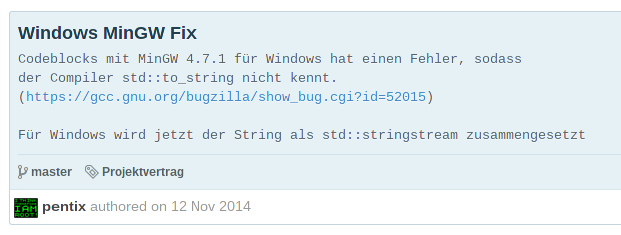
\includegraphics[scale=0.8]{img/e419eef.png}
\caption{Erläuterung in einem Commit}
\end{figure}

\subsection{Fehler in der Leveldatei}
Die Leveldatei war von Anfang an sehr Fehler anfällig. Da die Reihenfolge der Zahlen  genau stimmen muss. Da kann leicht ein Fehler unterlaufen. Die sind aber dann klar ersichtlich, da das ganze Bild ganz anders aus sieht als man erwartet hat. Man muss einfach die Leveldatei noch einemal überprüfen. Die Leveldatei ist auch ständig gewachsen, so dass man leicht einmal etwas vergessen konnte. Blöd ist einfach dass man sich keine Hinweise ins Dokument schreiben darf, weil sonst das ganze durcheinander kommt.

Bild

\subsection{Fehler beim Laser}
WIr haben ein weiteres testlevel erstellt und dieses mal sollte es mehrere Laser haben. Doch dies wollte nicht funktionieren, es funktionierte genau ein Laser. Die anderen waren zwar gezeichnet aber die Checkcollision-Funktion wollte nicht gehen. Da haben wir das ganze mehrere male durchgelesen. Bis jemandem aufgefallen ist, dass es immer nur der erste Laser ist, der funktionierte. Da fiel es uns dann auch wie Schuppen von den Augen, die eine Klammer war zu früh geschlossen worden. Danach lief es einwandfrei.

\subsection{Doppelter Tastendruck}
SFML gab an, dass eine Taste doppelt gedrückt wurde, obwohl sie nur einmal gedrückt wurde. Massnahme: Zeitliche Aussortierung

\subsection{Merge Conflicts}
git, unsere Versionskontrolle, ermöglichte es uns, parallel, in sogenannten Branches zu entwickeln. (Siehe Abbildung \ref{fig:branches} auf Seite \pageref{fig:branches}). Wir entwickelten neue Funktionen oft parallel und "mergten" (engl. to merge = zusammenführen) sie in unseren master-Zweig.
git nimmt alle Änderungen, die in beiden Zweigen seit dem letzten gemeinsamen Commit erstellt wurden, und erstellt daraus neue Dateien, die alle Änderungen,
also die Änderungen von beiden Zweigen beeinhalten. Es kann sein, dass nun 2 Personen gleichzeitig an derselben Stelle im Code etwas geändert haben. Zum Beispiel
hat der eine Entwickler eine Abfrage gelöscht, weil er sie nicht mehr brauchte, ein anderer Entwickler hat jedoch dieselbe Abfrage erweitert, da er sie benötigt.
git kann nun nicht mehr automatisch entscheiden wie der Code zusammenzuführen ist, bzw. wie die Versionen kombiniert sein sollen. Daraus resultiert ein Merge
Conflict. Git erstellt eine Datei, in der beide Versionen der Entwickler vorhanden sind und bittet den Entwickler, der den Code des anderen in seinen führen
will, um Hilfe. Unsere Konflikte waren meistens schnell gelöst, da sie nur zwei bis drei Zeilen betrafen, zum Beispiel wurde bei beiden Entwicklern
eine Variable unbenannt und man musste entscheiden, welche Version man wählt.\\
\\
Mühsam hingegen waren Konflikte, die mehrere Dateien betrafen, und in der 20 bis 30 Zeilen in einem Klammerwirrwar in Konflikt stehen. Da die Dateien und die Zeilen
logisch voneinander abhängen, musste man sehr umsichtig sein, und brauchte entsprechend viel Zeit und Geduld einen solchen Konflikt zu lösen. Es gab zum Glück kein
grosser Konflikt, der uns Probleme bereitete.
\newpage

\subsection{Paralleles Entwickeln des Kerns}
Obwohl wir bereits am Anfang parallel mit git entwickeln konnten, war es sehr schwierig, da noch gar kein Code vorhanden war,
und es zuerst galt, eine Basis zu entwickeln, auf der dann alle Programmieren konnten. Wir versuchten von Anfang an so zu programmieren,
dass wir später keine grossen Änderungen vornehmen mussten, um das Spiel um Laserschranken oder auch Musik zu erweitern.
\\
\\
Das gelang uns sehr gut, einzig die Levelklasse brauchte eine Restrukturierung, da die \textit{loadFromFile()}-Methode eine Leveldatei nicht nur mehr auslas,
sondern die Objekte auch gleich zeichnete. Da wir die Level aber speichern und nicht immer mehr komplett neu laden wollten, brauchten wir eine
Funktion, die es uns ermöglichte nur die Objekte in die Levelklasse zu laden und eine Funktion, die nur dazu da war, die gespeicherten Objekte zu zeichnen. So konnten wir Veränderungen an den Objekten in der Levelklasse abspeichern.
\\
\\
Ansonsten mussten wir am ganzen Kern nichts mehr ändern. Der grosse Vorteil, der sich dadurch ergab, war, dass jeder seine 
Funktionen kannte, und zum Beispiel problemlos Objekte erstellen konnte und diese auch auf Kollisionen mit dem Spieler überprüfen konnte.

\subsection{Mathematik}
Aufwand zum berechnen/ Logik

\subsection{Verfügbare Zeit}
Am Anfang des Projektunterrichts dachten wir, wir hätten mehr Zeit für die eigentliche Entwicklung. Wir mussten schlussendlich aber auch
sehr viel Zeit in die Disposition, den Projektvertrag und das Lernprotokoll stecken. Die Zeit, die uns für die Dokumentation und das Spiel
blieb, haben wir aber sehr intensiv genutzt. Die Kreise in Abbildung \ref{fig:punchcard} zeigen additiv, wie viel und wann seit Projektbeginn programmiert wurde.

\begin{figure}[h]
\centering
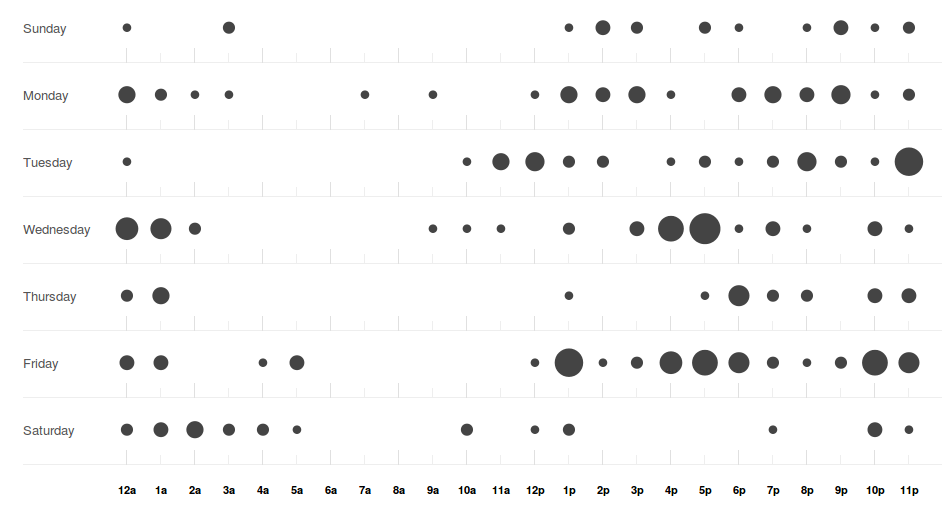
\includegraphics[scale=0.4]{img/punchcard.png}
\caption{Punchcard - Darstellung der Entwicklungszeiten}
\label{fig:punchcard}
\end{figure}

\section{Das Spiel}
\subsection{Das Spielprinzip}
Das Spielprinzip ist einfach: Als Einbrecher versucht man in ein Haus einzubrechen, und dabei keinen Lärm zu verursachen, Laserschranken auszuweichen
und dies je nach Spielmodus möglichst schnell, oder sehr ausgiebig.

\subsection{Spielmodi}
Wir haben unsere Level verschieden erstellt:
\begin{itemize}
\item Zeitdruck: Die Zeit wurde bewusst sehr knapp gewählt, und man musste die Schätze finden, bevor diese ablief.
\item Suche: Die Schätze waren im ganzen Haus versteckt und gut mit Laserschranken gesichert.
\item Schatz: Es gab nur einen einzigen, im dunklen gut versteckten Schatz.
\end{itemize}

\newpage
\section{Diskussion / Reflexion}


\newpage
\section{Mögliche Erweiterungen / Ausblick}
Wir wissen wir sind immer noch einige Schritte von einem kompletten Game entfernt. Es fehlen schon alleine die verschiedenen Levels. Dazu kommt, dass wir auch noch Gegner einbauen möchten. So dass man Gegner hat die herumlaufen und einem entdecken können, das könnte zum Beispiel ein Hund sein. Wir möchten auch, dass der Schallpegel erhöht wird, im Falle von einer Kollision mit einer Mauer. 	
\\ 	
\\ 	
Wir werden weiterhin an dieem Spiel weiter schreiben, da es uns doch sehr gefällt zu programmieren, aber auch weil uns der Ehrgeiz gefasst hat. Wir wollen ein richtiges Spiel zum laufen bekommen. Unsere Wunschvorstellung wäre, dass wir es dann einmal auf eine Online Gamerplatform stellen könnten. So dass es dann auch aktiv gespielt wird. 


\clearpage
\part{Anhang}
\listoffigures

\clearpage

\addcontentsline{toc}{section}{Literatur}
\printbibliography

\clearpage

\addcontentsline{toc}{section}{Antiplagiatserklärung}
\section*{Antiplagiatserklärung}
Wir versichern hiermit, die vorliegende Arbeit, inklusive des entstandenen Spiels
selber, ohne fremde Hilfe verfasst zu haben. Alle Quellen, die zur Erstellung
der Arbeit verwendet wurden, wurden in der Literaturliste aufgeführt.
\\\\\\
\textbf{Aarau, der \today}\\

% Hier kommen die Unterschriten hin
\vspace{1 cm} 
\begin{tabular}{p{5cm}p{.5cm}l}
\dotfill \\ 
\begin{center}
Gabriel Gavrilas

\end{center}\end{tabular}% 
\hfill 
\begin{tabular}{p{5cm}p{.5cm}l}
\dotfill \\ 
\begin{center}
Jan Kunzmann

\end{center}\end{tabular}% 
\hfill 
\begin{tabular}{p{5cm}p{.5cm}l}
\dotfill \\ 
\begin{center}
Patrick Eigensatz
\end{center}
\end{tabular}% 
  


\end{document}
